% Options for packages loaded elsewhere
\PassOptionsToPackage{unicode}{hyperref}
\PassOptionsToPackage{hyphens}{url}
%
\documentclass[
]{article}
\usepackage{amsmath,amssymb}
\usepackage{iftex}
\ifPDFTeX
  \usepackage[T1]{fontenc}
  \usepackage[utf8]{inputenc}
  \usepackage{textcomp} % provide euro and other symbols
\else % if luatex or xetex
  \usepackage{unicode-math} % this also loads fontspec
  \defaultfontfeatures{Scale=MatchLowercase}
  \defaultfontfeatures[\rmfamily]{Ligatures=TeX,Scale=1}
\fi
\usepackage{lmodern}
\ifPDFTeX\else
  % xetex/luatex font selection
\fi
% Use upquote if available, for straight quotes in verbatim environments
\IfFileExists{upquote.sty}{\usepackage{upquote}}{}
\IfFileExists{microtype.sty}{% use microtype if available
  \usepackage[]{microtype}
  \UseMicrotypeSet[protrusion]{basicmath} % disable protrusion for tt fonts
}{}
\makeatletter
\@ifundefined{KOMAClassName}{% if non-KOMA class
  \IfFileExists{parskip.sty}{%
    \usepackage{parskip}
  }{% else
    \setlength{\parindent}{0pt}
    \setlength{\parskip}{6pt plus 2pt minus 1pt}}
}{% if KOMA class
  \KOMAoptions{parskip=half}}
\makeatother
\usepackage{xcolor}
\usepackage[margin=1in]{geometry}
\usepackage{color}
\usepackage{fancyvrb}
\newcommand{\VerbBar}{|}
\newcommand{\VERB}{\Verb[commandchars=\\\{\}]}
\DefineVerbatimEnvironment{Highlighting}{Verbatim}{commandchars=\\\{\}}
% Add ',fontsize=\small' for more characters per line
\usepackage{framed}
\definecolor{shadecolor}{RGB}{248,248,248}
\newenvironment{Shaded}{\begin{snugshade}}{\end{snugshade}}
\newcommand{\AlertTok}[1]{\textcolor[rgb]{0.94,0.16,0.16}{#1}}
\newcommand{\AnnotationTok}[1]{\textcolor[rgb]{0.56,0.35,0.01}{\textbf{\textit{#1}}}}
\newcommand{\AttributeTok}[1]{\textcolor[rgb]{0.13,0.29,0.53}{#1}}
\newcommand{\BaseNTok}[1]{\textcolor[rgb]{0.00,0.00,0.81}{#1}}
\newcommand{\BuiltInTok}[1]{#1}
\newcommand{\CharTok}[1]{\textcolor[rgb]{0.31,0.60,0.02}{#1}}
\newcommand{\CommentTok}[1]{\textcolor[rgb]{0.56,0.35,0.01}{\textit{#1}}}
\newcommand{\CommentVarTok}[1]{\textcolor[rgb]{0.56,0.35,0.01}{\textbf{\textit{#1}}}}
\newcommand{\ConstantTok}[1]{\textcolor[rgb]{0.56,0.35,0.01}{#1}}
\newcommand{\ControlFlowTok}[1]{\textcolor[rgb]{0.13,0.29,0.53}{\textbf{#1}}}
\newcommand{\DataTypeTok}[1]{\textcolor[rgb]{0.13,0.29,0.53}{#1}}
\newcommand{\DecValTok}[1]{\textcolor[rgb]{0.00,0.00,0.81}{#1}}
\newcommand{\DocumentationTok}[1]{\textcolor[rgb]{0.56,0.35,0.01}{\textbf{\textit{#1}}}}
\newcommand{\ErrorTok}[1]{\textcolor[rgb]{0.64,0.00,0.00}{\textbf{#1}}}
\newcommand{\ExtensionTok}[1]{#1}
\newcommand{\FloatTok}[1]{\textcolor[rgb]{0.00,0.00,0.81}{#1}}
\newcommand{\FunctionTok}[1]{\textcolor[rgb]{0.13,0.29,0.53}{\textbf{#1}}}
\newcommand{\ImportTok}[1]{#1}
\newcommand{\InformationTok}[1]{\textcolor[rgb]{0.56,0.35,0.01}{\textbf{\textit{#1}}}}
\newcommand{\KeywordTok}[1]{\textcolor[rgb]{0.13,0.29,0.53}{\textbf{#1}}}
\newcommand{\NormalTok}[1]{#1}
\newcommand{\OperatorTok}[1]{\textcolor[rgb]{0.81,0.36,0.00}{\textbf{#1}}}
\newcommand{\OtherTok}[1]{\textcolor[rgb]{0.56,0.35,0.01}{#1}}
\newcommand{\PreprocessorTok}[1]{\textcolor[rgb]{0.56,0.35,0.01}{\textit{#1}}}
\newcommand{\RegionMarkerTok}[1]{#1}
\newcommand{\SpecialCharTok}[1]{\textcolor[rgb]{0.81,0.36,0.00}{\textbf{#1}}}
\newcommand{\SpecialStringTok}[1]{\textcolor[rgb]{0.31,0.60,0.02}{#1}}
\newcommand{\StringTok}[1]{\textcolor[rgb]{0.31,0.60,0.02}{#1}}
\newcommand{\VariableTok}[1]{\textcolor[rgb]{0.00,0.00,0.00}{#1}}
\newcommand{\VerbatimStringTok}[1]{\textcolor[rgb]{0.31,0.60,0.02}{#1}}
\newcommand{\WarningTok}[1]{\textcolor[rgb]{0.56,0.35,0.01}{\textbf{\textit{#1}}}}
\usepackage{graphicx}
\makeatletter
\def\maxwidth{\ifdim\Gin@nat@width>\linewidth\linewidth\else\Gin@nat@width\fi}
\def\maxheight{\ifdim\Gin@nat@height>\textheight\textheight\else\Gin@nat@height\fi}
\makeatother
% Scale images if necessary, so that they will not overflow the page
% margins by default, and it is still possible to overwrite the defaults
% using explicit options in \includegraphics[width, height, ...]{}
\setkeys{Gin}{width=\maxwidth,height=\maxheight,keepaspectratio}
% Set default figure placement to htbp
\makeatletter
\def\fps@figure{htbp}
\makeatother
\setlength{\emergencystretch}{3em} % prevent overfull lines
\providecommand{\tightlist}{%
  \setlength{\itemsep}{0pt}\setlength{\parskip}{0pt}}
\setcounter{secnumdepth}{-\maxdimen} % remove section numbering
\usepackage{fvextra}
\DefineVerbatimEnvironment{Highlighting}{Verbatim}{breaklines,commandchars=\\\{\}}
\ifLuaTeX
  \usepackage{selnolig}  % disable illegal ligatures
\fi
\usepackage{bookmark}
\IfFileExists{xurl.sty}{\usepackage{xurl}}{} % add URL line breaks if available
\urlstyle{same}
\hypersetup{
  pdftitle={SDA Group Submission Assignment Assign3},
  pdfauthor={MengliFeng (2720589) and PepijnVanOostveen (2801582)},
  hidelinks,
  pdfcreator={LaTeX via pandoc}}

\title{SDA Group Submission Assignment Assign3}
\usepackage{etoolbox}
\makeatletter
\providecommand{\subtitle}[1]{% add subtitle to \maketitle
  \apptocmd{\@title}{\par {\large #1 \par}}{}{}
}
\makeatother
\subtitle{Group Gr18}
\author{MengliFeng (2720589) and PepijnVanOostveen (2801582)}
\date{}

\begin{document}
\maketitle

\section{Exercise 1}\label{exercise-1}

\subsection{a.}\label{a.}

\begin{Shaded}
\begin{Highlighting}[]
\CommentTok{\# Set seed for reproducibility}
\FunctionTok{set.seed}\NormalTok{(}\DecValTok{123}\NormalTok{)}

\CommentTok{\# Generate random sample from t{-}distribution with 3 degrees of freedom}
\NormalTok{n }\OtherTok{\textless{}{-}} \DecValTok{20}
\NormalTok{sample\_data }\OtherTok{\textless{}{-}} \FunctionTok{rt}\NormalTok{(n, }\AttributeTok{df =} \DecValTok{3}\NormalTok{)}

\CommentTok{\# Define different kernel types and colors}
\NormalTok{kernels }\OtherTok{\textless{}{-}} \FunctionTok{c}\NormalTok{(}\StringTok{"gaussian"}\NormalTok{, }\StringTok{"epanechnikov"}\NormalTok{, }\StringTok{"rectangular"}\NormalTok{, }\StringTok{"triangular"}\NormalTok{)}
\NormalTok{colors\_kernels }\OtherTok{\textless{}{-}} \FunctionTok{c}\NormalTok{(}\StringTok{"red"}\NormalTok{, }\StringTok{"blue"}\NormalTok{, }\StringTok{"green"}\NormalTok{, }\StringTok{"purple"}\NormalTok{)}

\CommentTok{\# Define different bandwidth choices and colors}
\NormalTok{bandwidths }\OtherTok{\textless{}{-}} \FunctionTok{c}\NormalTok{(}\FunctionTok{density}\NormalTok{(sample\_data)}\SpecialCharTok{$}\NormalTok{bw, }\FloatTok{0.3}\NormalTok{, }\FloatTok{1.5}\NormalTok{)}
\NormalTok{colors\_bandwidths }\OtherTok{\textless{}{-}} \FunctionTok{c}\NormalTok{(}\StringTok{"red"}\NormalTok{, }\StringTok{"blue"}\NormalTok{, }\StringTok{"green"}\NormalTok{)}

\CommentTok{\# Adjust plot margins to make space for legends}
\FunctionTok{par}\NormalTok{(}\AttributeTok{mfrow =} \FunctionTok{c}\NormalTok{(}\DecValTok{1}\NormalTok{, }\DecValTok{2}\NormalTok{), }\AttributeTok{mar =} \FunctionTok{c}\NormalTok{(}\DecValTok{5}\NormalTok{, }\DecValTok{4}\NormalTok{, }\DecValTok{6}\NormalTok{, }\DecValTok{4}\NormalTok{))  }\CommentTok{\# Extra right margin for the legend}

\CommentTok{\# Plot histogram with different kernel choices}
\FunctionTok{hist}\NormalTok{(sample\_data, }\AttributeTok{probability =} \ConstantTok{TRUE}\NormalTok{, }\AttributeTok{main =} \StringTok{"Kernels"}\NormalTok{, }\AttributeTok{col =} \StringTok{"lightgray"}\NormalTok{, }\AttributeTok{border =} \StringTok{"black"}\NormalTok{)}

\ControlFlowTok{for}\NormalTok{ (i }\ControlFlowTok{in} \FunctionTok{seq\_along}\NormalTok{(kernels)) \{}
  \FunctionTok{lines}\NormalTok{(}\FunctionTok{density}\NormalTok{(sample\_data, }\AttributeTok{kernel =}\NormalTok{ kernels[i]), }\AttributeTok{col =}\NormalTok{ colors\_kernels[i], }\AttributeTok{lwd =} \DecValTok{2}\NormalTok{)}
\NormalTok{\}}

\CommentTok{\# Add legend outside the plot}
\FunctionTok{legend}\NormalTok{(}\StringTok{"topright"}\NormalTok{, }\AttributeTok{inset =} \FunctionTok{c}\NormalTok{(}\SpecialCharTok{{-}}\FloatTok{0.3}\NormalTok{, }\DecValTok{0}\NormalTok{), }\AttributeTok{legend =}\NormalTok{ kernels, }\AttributeTok{col =}\NormalTok{ colors\_kernels, }\AttributeTok{lwd =} \DecValTok{2}\NormalTok{, }\AttributeTok{cex =} \FloatTok{0.5}\NormalTok{, }\AttributeTok{title =} \StringTok{"Kernels"}\NormalTok{, }\AttributeTok{xpd =} \ConstantTok{TRUE}\NormalTok{)}

\CommentTok{\# Plot histogram with different bandwidth choices}
\FunctionTok{hist}\NormalTok{(sample\_data, }\AttributeTok{probability =} \ConstantTok{TRUE}\NormalTok{, }\AttributeTok{main =} \StringTok{"Bandwidths (Gaussian)"}\NormalTok{, }\AttributeTok{col =} \StringTok{"lightgray"}\NormalTok{, }\AttributeTok{border =} \StringTok{"black"}\NormalTok{)}

\ControlFlowTok{for}\NormalTok{ (i }\ControlFlowTok{in} \FunctionTok{seq\_along}\NormalTok{(bandwidths)) \{}
  \FunctionTok{lines}\NormalTok{(}\FunctionTok{density}\NormalTok{(sample\_data, }\AttributeTok{bw =}\NormalTok{ bandwidths[i]), }\AttributeTok{col =}\NormalTok{ colors\_bandwidths[i], }\AttributeTok{lwd =} \DecValTok{2}\NormalTok{)}
\NormalTok{\}}

\CommentTok{\# Add legend outside the plot}
\FunctionTok{legend}\NormalTok{(}\StringTok{"topright"}\NormalTok{, }\AttributeTok{inset =} \FunctionTok{c}\NormalTok{(}\SpecialCharTok{{-}}\FloatTok{0.3}\NormalTok{, }\DecValTok{0}\NormalTok{), }\AttributeTok{legend =} \FunctionTok{paste}\NormalTok{(}\StringTok{"bw ="}\NormalTok{, }\FunctionTok{round}\NormalTok{(bandwidths, }\DecValTok{2}\NormalTok{)), }\AttributeTok{col =}\NormalTok{ colors\_bandwidths, }\AttributeTok{lwd =} \DecValTok{2}\NormalTok{, }\AttributeTok{cex =} \FloatTok{0.5}\NormalTok{,}
       \AttributeTok{title =} \StringTok{"Bandwidths"}\NormalTok{, }\AttributeTok{xpd =} \ConstantTok{TRUE}\NormalTok{)}

\CommentTok{\# {-}{-}{-} Add an Overall Title {-}{-}{-}}
\FunctionTok{mtext}\NormalTok{(}\StringTok{"Density Estimation with different kernels and kernel bandwidths"}\NormalTok{,}\AttributeTok{line =} \DecValTok{4}\NormalTok{, }\AttributeTok{cex =} \DecValTok{1}\NormalTok{, }\AttributeTok{font =} \DecValTok{1}\NormalTok{, }\AttributeTok{adj =} \DecValTok{1}\NormalTok{)}
\end{Highlighting}
\end{Shaded}

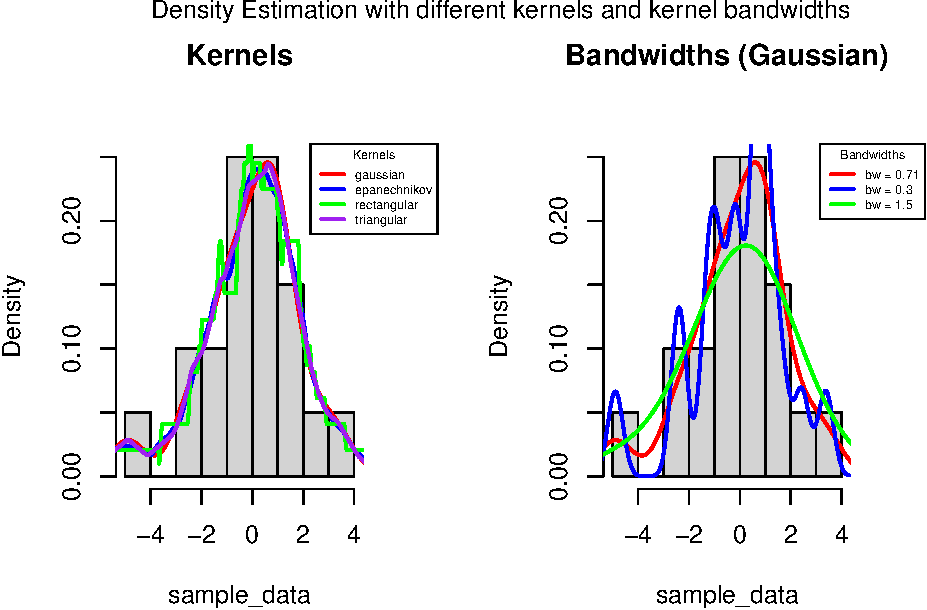
\includegraphics{SDA_submission_template_files/figure-latex/unnamed-chunk-1-1.pdf}

\subsection{b.}\label{b.}

From the generated plots, we can observe: • Effect of Kernel Choice:
Different kernels produce similar overall shapes, but their smoothness
varies slightly. The Gaussian kernel is the smoothest, while the
rectangular kernel has more abrupt changes. • Effect of Bandwidth
Choice: The bandwidth has a much larger influence than the kernel. A
smaller bandwidth (0.3) captures more fluctuations in the data, while a
larger bandwidth (1.5) smooths out more features. • Key Influence:
Bandwidth choice has a bigger impact on the estimator compared to kernel
choice. \#\# c.

\begin{Shaded}
\begin{Highlighting}[]
\NormalTok{h\_opt }\OtherTok{\textless{}{-}} \ControlFlowTok{function}\NormalTok{(x) \{}
\NormalTok{  sigma\_hat }\OtherTok{\textless{}{-}} \FunctionTok{min}\NormalTok{(}\FunctionTok{sd}\NormalTok{(x), }\FunctionTok{IQR}\NormalTok{(x) }\SpecialCharTok{/} \FloatTok{1.34}\NormalTok{)  }\CommentTok{\# Compute standard deviation and interquartile range}
\NormalTok{  h\_optimal }\OtherTok{\textless{}{-}} \FloatTok{1.06} \SpecialCharTok{*}\NormalTok{ sigma\_hat }\SpecialCharTok{*} \FunctionTok{length}\NormalTok{(x)}\SpecialCharTok{\^{}}\NormalTok{(}\SpecialCharTok{{-}}\DecValTok{1}\SpecialCharTok{/}\DecValTok{5}\NormalTok{)  }\CommentTok{\# Optimal bandwidth formula}
  \FunctionTok{return}\NormalTok{(h\_optimal)}
\NormalTok{\}}

\CommentTok{\# Compute optimal bandwidth for the sample}
\NormalTok{h\_opt\_value }\OtherTok{\textless{}{-}} \FunctionTok{h\_opt}\NormalTok{(sample\_data)}

\CommentTok{\# Compare with R\textquotesingle{}s default bandwidth}
\NormalTok{default\_bw }\OtherTok{\textless{}{-}} \FunctionTok{density}\NormalTok{(sample\_data)}\SpecialCharTok{$}\NormalTok{bw}

\CommentTok{\# Print results}
\FunctionTok{cat}\NormalTok{(}\StringTok{"Optimal Bandwidth (h\_opt):"}\NormalTok{, h\_opt\_value, }\StringTok{"}\SpecialCharTok{\textbackslash{}n}\StringTok{"}\NormalTok{)}
\end{Highlighting}
\end{Shaded}

\begin{verbatim}
## Optimal Bandwidth (h_opt): 0.831087
\end{verbatim}

\begin{Shaded}
\begin{Highlighting}[]
\FunctionTok{cat}\NormalTok{(}\StringTok{"Default R Bandwidth:"}\NormalTok{, default\_bw, }\StringTok{"}\SpecialCharTok{\textbackslash{}n}\StringTok{"}\NormalTok{)}
\end{Highlighting}
\end{Shaded}

\begin{verbatim}
## Default R Bandwidth: 0.7056399
\end{verbatim}

\section{Exercise 2}\label{exercise-2}

\subsection{a.}\label{a.-1}

\subsection{b.}\label{b.-1}

\subsection{c.}\label{c.}

\end{document}
